% Options for packages loaded elsewhere
\PassOptionsToPackage{unicode}{hyperref}
\PassOptionsToPackage{hyphens}{url}
%
\documentclass[
  ignorenonframetext,
  aspectratio=169,
]{beamer}
\usepackage{pgfpages}
\setbeamertemplate{caption}[numbered]
\setbeamertemplate{caption label separator}{: }
\setbeamercolor{caption name}{fg=normal text.fg}
\beamertemplatenavigationsymbolsempty
% Prevent slide breaks in the middle of a paragraph
\widowpenalties 1 10000
\raggedbottom
\setbeamertemplate{part page}{
  \centering
  \begin{beamercolorbox}[sep=16pt,center]{part title}
    \usebeamerfont{part title}\insertpart\par
  \end{beamercolorbox}
}
\setbeamertemplate{section page}{
  \centering
  \begin{beamercolorbox}[sep=12pt,center]{part title}
    \usebeamerfont{section title}\insertsection\par
  \end{beamercolorbox}
}
\setbeamertemplate{subsection page}{
  \centering
  \begin{beamercolorbox}[sep=8pt,center]{part title}
    \usebeamerfont{subsection title}\insertsubsection\par
  \end{beamercolorbox}
}
\AtBeginPart{
  \frame{\partpage}
}
\AtBeginSection{
  \ifbibliography
  \else
    \frame{\sectionpage}
  \fi
}
\AtBeginSubsection{
  \frame{\subsectionpage}
}

\usepackage{amsmath,amssymb}
\usepackage{iftex}
\ifPDFTeX
  \usepackage[T1]{fontenc}
  \usepackage[utf8]{inputenc}
  \usepackage{textcomp} % provide euro and other symbols
\else % if luatex or xetex
  \usepackage{unicode-math}
  \defaultfontfeatures{Scale=MatchLowercase}
  \defaultfontfeatures[\rmfamily]{Ligatures=TeX,Scale=1}
\fi
\usepackage{lmodern}
\ifPDFTeX\else  
    % xetex/luatex font selection
  \setmonofont[Scale=0.35]{Menlo}
\fi
% Use upquote if available, for straight quotes in verbatim environments
\IfFileExists{upquote.sty}{\usepackage{upquote}}{}
\IfFileExists{microtype.sty}{% use microtype if available
  \usepackage[]{microtype}
  \UseMicrotypeSet[protrusion]{basicmath} % disable protrusion for tt fonts
}{}
\makeatletter
\@ifundefined{KOMAClassName}{% if non-KOMA class
  \IfFileExists{parskip.sty}{%
    \usepackage{parskip}
  }{% else
    \setlength{\parindent}{0pt}
    \setlength{\parskip}{6pt plus 2pt minus 1pt}}
}{% if KOMA class
  \KOMAoptions{parskip=half}}
\makeatother
\usepackage{xcolor}
\newif\ifbibliography
\setlength{\emergencystretch}{3em} % prevent overfull lines
\setcounter{secnumdepth}{-\maxdimen} % remove section numbering

\usepackage{color}
\usepackage{fancyvrb}
\newcommand{\VerbBar}{|}
\newcommand{\VERB}{\Verb[commandchars=\\\{\}]}
\DefineVerbatimEnvironment{Highlighting}{Verbatim}{commandchars=\\\{\}}
% Add ',fontsize=\small' for more characters per line
\usepackage{framed}
\definecolor{shadecolor}{RGB}{241,243,245}
\newenvironment{Shaded}{\begin{snugshade}}{\end{snugshade}}
\newcommand{\AlertTok}[1]{\textcolor[rgb]{0.68,0.00,0.00}{#1}}
\newcommand{\AnnotationTok}[1]{\textcolor[rgb]{0.37,0.37,0.37}{#1}}
\newcommand{\AttributeTok}[1]{\textcolor[rgb]{0.40,0.45,0.13}{#1}}
\newcommand{\BaseNTok}[1]{\textcolor[rgb]{0.68,0.00,0.00}{#1}}
\newcommand{\BuiltInTok}[1]{\textcolor[rgb]{0.00,0.23,0.31}{#1}}
\newcommand{\CharTok}[1]{\textcolor[rgb]{0.13,0.47,0.30}{#1}}
\newcommand{\CommentTok}[1]{\textcolor[rgb]{0.37,0.37,0.37}{#1}}
\newcommand{\CommentVarTok}[1]{\textcolor[rgb]{0.37,0.37,0.37}{\textit{#1}}}
\newcommand{\ConstantTok}[1]{\textcolor[rgb]{0.56,0.35,0.01}{#1}}
\newcommand{\ControlFlowTok}[1]{\textcolor[rgb]{0.00,0.23,0.31}{#1}}
\newcommand{\DataTypeTok}[1]{\textcolor[rgb]{0.68,0.00,0.00}{#1}}
\newcommand{\DecValTok}[1]{\textcolor[rgb]{0.68,0.00,0.00}{#1}}
\newcommand{\DocumentationTok}[1]{\textcolor[rgb]{0.37,0.37,0.37}{\textit{#1}}}
\newcommand{\ErrorTok}[1]{\textcolor[rgb]{0.68,0.00,0.00}{#1}}
\newcommand{\ExtensionTok}[1]{\textcolor[rgb]{0.00,0.23,0.31}{#1}}
\newcommand{\FloatTok}[1]{\textcolor[rgb]{0.68,0.00,0.00}{#1}}
\newcommand{\FunctionTok}[1]{\textcolor[rgb]{0.28,0.35,0.67}{#1}}
\newcommand{\ImportTok}[1]{\textcolor[rgb]{0.00,0.46,0.62}{#1}}
\newcommand{\InformationTok}[1]{\textcolor[rgb]{0.37,0.37,0.37}{#1}}
\newcommand{\KeywordTok}[1]{\textcolor[rgb]{0.00,0.23,0.31}{#1}}
\newcommand{\NormalTok}[1]{\textcolor[rgb]{0.00,0.23,0.31}{#1}}
\newcommand{\OperatorTok}[1]{\textcolor[rgb]{0.37,0.37,0.37}{#1}}
\newcommand{\OtherTok}[1]{\textcolor[rgb]{0.00,0.23,0.31}{#1}}
\newcommand{\PreprocessorTok}[1]{\textcolor[rgb]{0.68,0.00,0.00}{#1}}
\newcommand{\RegionMarkerTok}[1]{\textcolor[rgb]{0.00,0.23,0.31}{#1}}
\newcommand{\SpecialCharTok}[1]{\textcolor[rgb]{0.37,0.37,0.37}{#1}}
\newcommand{\SpecialStringTok}[1]{\textcolor[rgb]{0.13,0.47,0.30}{#1}}
\newcommand{\StringTok}[1]{\textcolor[rgb]{0.13,0.47,0.30}{#1}}
\newcommand{\VariableTok}[1]{\textcolor[rgb]{0.07,0.07,0.07}{#1}}
\newcommand{\VerbatimStringTok}[1]{\textcolor[rgb]{0.13,0.47,0.30}{#1}}
\newcommand{\WarningTok}[1]{\textcolor[rgb]{0.37,0.37,0.37}{\textit{#1}}}

\providecommand{\tightlist}{%
  \setlength{\itemsep}{0pt}\setlength{\parskip}{0pt}}\usepackage{longtable,booktabs,array}
\usepackage{calc} % for calculating minipage widths
\usepackage{caption}
% Make caption package work with longtable
\makeatletter
\def\fnum@table{\tablename~\thetable}
\makeatother
\usepackage{graphicx}
\makeatletter
\def\maxwidth{\ifdim\Gin@nat@width>\linewidth\linewidth\else\Gin@nat@width\fi}
\def\maxheight{\ifdim\Gin@nat@height>\textheight\textheight\else\Gin@nat@height\fi}
\makeatother
% Scale images if necessary, so that they will not overflow the page
% margins by default, and it is still possible to overwrite the defaults
% using explicit options in \includegraphics[width, height, ...]{}
\setkeys{Gin}{width=\maxwidth,height=\maxheight,keepaspectratio}
% Set default figure placement to htbp
\makeatletter
\def\fps@figure{htbp}
\makeatother

\makeatletter
\makeatother
\makeatletter
\makeatother
\makeatletter
\@ifpackageloaded{caption}{}{\usepackage{caption}}
\AtBeginDocument{%
\ifdefined\contentsname
  \renewcommand*\contentsname{Table of contents}
\else
  \newcommand\contentsname{Table of contents}
\fi
\ifdefined\listfigurename
  \renewcommand*\listfigurename{List of Figures}
\else
  \newcommand\listfigurename{List of Figures}
\fi
\ifdefined\listtablename
  \renewcommand*\listtablename{List of Tables}
\else
  \newcommand\listtablename{List of Tables}
\fi
\ifdefined\figurename
  \renewcommand*\figurename{Figure}
\else
  \newcommand\figurename{Figure}
\fi
\ifdefined\tablename
  \renewcommand*\tablename{Table}
\else
  \newcommand\tablename{Table}
\fi
}
\@ifpackageloaded{float}{}{\usepackage{float}}
\floatstyle{ruled}
\@ifundefined{c@chapter}{\newfloat{codelisting}{h}{lop}}{\newfloat{codelisting}{h}{lop}[chapter]}
\floatname{codelisting}{Listing}
\newcommand*\listoflistings{\listof{codelisting}{List of Listings}}
\makeatother
\makeatletter
\@ifpackageloaded{caption}{}{\usepackage{caption}}
\@ifpackageloaded{subcaption}{}{\usepackage{subcaption}}
\makeatother
\makeatletter
\@ifpackageloaded{tcolorbox}{}{\usepackage[skins,breakable]{tcolorbox}}
\makeatother
\makeatletter
\@ifundefined{shadecolor}{\definecolor{shadecolor}{rgb}{.97, .97, .97}}
\makeatother
\makeatletter
\makeatother
\makeatletter
\makeatother
\ifLuaTeX
  \usepackage{selnolig}  % disable illegal ligatures
\fi
\usepackage[]{natbib}
\bibliographystyle{plainnat}
\IfFileExists{bookmark.sty}{\usepackage{bookmark}}{\usepackage{hyperref}}
\IfFileExists{xurl.sty}{\usepackage{xurl}}{} % add URL line breaks if available
\urlstyle{same} % disable monospaced font for URLs
\hypersetup{
  pdftitle={Reproducible Global N},
  pdfauthor={Arturo Torres},
  hidelinks,
  pdfcreator={LaTeX via pandoc}}

\title{Reproducible Global N}
\subtitle{Reproducible Spatial Analysis for Charting Nitrogen Dynamics
in Global Wheat Production}
\author{Arturo Torres}
\date{Tuesday, October 17, 2023}

\begin{document}
\frame{\titlepage}
\ifdefined\Shaded\renewenvironment{Shaded}{\begin{tcolorbox}[interior hidden, borderline west={3pt}{0pt}{shadecolor}, enhanced, breakable, sharp corners, frame hidden, boxrule=0pt]}{\end{tcolorbox}}\fi

\begin{frame}{Goal}
\protect\hypertarget{goal}{}
\begin{itemize}[<+->]
\item
  Following the indications, the goal of this reproducible code is to
  (IIASA-BNR, 2023, assignment):

  \begin{itemize}[<+->]
  \item
    ``Combine various datasets to generate indictors of nitrogen loss to
    the environment associated with wheat production at various spatial
    scales''
  \item
    ``Provide graphical representations and conduct simple comparisons
    across a few countries''
  \item
    ``Provide a reproducible code associated to these tasks.''
  \end{itemize}
\end{itemize}
\end{frame}

\begin{frame}{Task 1}
\protect\hypertarget{task-1}{}
\begin{itemize}[<+->]
\item
  Using SPAM raster data \citep{wood-sichra_spatial_2016}, a new raster
  at the same resolution, containing wheat production volume (in million
  tons Mt) is produced.
\item
  Global scale in a raster format (5 arcminute spatial resolution)
  estimates of yield (r\_y) in Kg/Ha, physical area (r\_a) in Ha and
  harvested area (r\_h) in Ha for the year 2005 are available.
\end{itemize}

\linespread{0.5}

\linespread{2}
\end{frame}

\begin{frame}[fragile]{Reading SPAM data}
\protect\hypertarget{reading-spam-data}{}
\linespread{0.5}

\begin{Shaded}
\begin{Highlighting}[]
\NormalTok{spam\_data }\OtherTok{=} \FunctionTok{list}\NormalTok{(}\StringTok{"yield"} \OtherTok{=} \FunctionTok{rast}\NormalTok{(}\StringTok{"data/SPAM\_2005\_v3.2/SPAM2005V3r2\_global\_Y\_TA\_WHEA\_A.tif"}\NormalTok{),}
                 \StringTok{"harvested\_area"} \OtherTok{=} \FunctionTok{rast}\NormalTok{(}\StringTok{"data/SPAM\_2005\_v3.2/SPAM2005V3r2\_global\_H\_TA\_WHEA\_A.tif"}\NormalTok{),}
                 \StringTok{"physical\_area"} \OtherTok{=} \FunctionTok{rast}\NormalTok{(}\StringTok{"data/SPAM\_2005\_v3.2/SPAM2005V3r2\_global\_A\_TA\_WHEA\_A.tif"}\NormalTok{))}
\end{Highlighting}
\end{Shaded}

\linespread{2}

\linespread{0.5}

\begin{Shaded}
\begin{Highlighting}[]
\FunctionTok{str}\NormalTok{(spam\_data)   }
\end{Highlighting}
\end{Shaded}

\begin{verbatim}
List of 3
 $ yield         :S4 class 'SpatRaster' [package "terra"]
 $ harvested_area:S4 class 'SpatRaster' [package "terra"]
 $ physical_area :S4 class 'SpatRaster' [package "terra"]
\end{verbatim}

\begin{Shaded}
\begin{Highlighting}[]
\NormalTok{spam\_data[[}\StringTok{\textquotesingle{}yield\textquotesingle{}}\NormalTok{]]}
\end{Highlighting}
\end{Shaded}

\begin{verbatim}
class       : SpatRaster 
dimensions  : 1853, 4320, 1  (nrow, ncol, nlyr)
resolution  : 0.08333333, 0.08333333  (x, y)
extent      : -180, 180, -64.41667, 90  (xmin, xmax, ymin, ymax)
coord. ref. : lon/lat WGS 84 (EPSG:4326) 
source      : SPAM2005V3r2_global_Y_TA_WHEA_A.tif 
name        : SPAM2005V3r2_global_Y_TA_WHEA_A 
min value   :                               0 
max value   :                           19429 
\end{verbatim}

\linespread{2}
\end{frame}

\begin{frame}{Calculate Wheat Production}
\protect\hypertarget{calculate-wheat-production}{}
\begin{itemize}[<+->]
\item
  Calculate wheat production by multiplying the raster layers for yield
  (in Kg/Ha) and harvested area (in Ha) using the * operator:

  \begin{itemize}[<+->]
  \tightlist
  \item
    wheat\_production = spam\_data{[}{[}``yield''{]}{]} *
    spam\_data{[}{[}``harvested\_area''{]}{]}
  \end{itemize}
\item
  Convert Units: The resulting values are in Kg, so it is needed to
  convert them to million tons (Mt). Assuming 1 ton is equal to 1,000
  Kg, it is possible to use the following:

  \begin{itemize}[<+->]
  \tightlist
  \item
    wheat\_production\_Mt = wheat\_production / (1e3 * 1e6)
  \end{itemize}
\end{itemize}
\end{frame}

\begin{frame}[fragile]{Calculate Wheat Production}
\protect\hypertarget{calculate-wheat-production-1}{}
\begin{itemize}[<+->]
\tightlist
\item
  A global map is created and the raster is exported in a geotif format:
\end{itemize}

\begin{columns}[T]
\begin{column}{0.8\textwidth}
\linespread{0.5}

\begin{Shaded}
\begin{Highlighting}[]
\NormalTok{wheat\_production }\OtherTok{=}\NormalTok{ spam\_data[[}\StringTok{"yield"}\NormalTok{]] }\SpecialCharTok{*}\NormalTok{ spam\_data[[}\StringTok{"harvested\_area"}\NormalTok{]]}
\NormalTok{wheat\_production\_Mt }\OtherTok{\textless{}{-}}\NormalTok{ wheat\_production }\SpecialCharTok{/}\NormalTok{ (}\FloatTok{1e9}\NormalTok{)}
\end{Highlighting}
\end{Shaded}

\linespread{2}

\linespread{0.5}

\begin{Shaded}
\begin{Highlighting}[]
\FunctionTok{plot}\NormalTok{(wheat\_production\_Mt, }\AttributeTok{col =} \FunctionTok{terrain.colors}\NormalTok{(}\DecValTok{10}\NormalTok{, }\AttributeTok{rev=}\ConstantTok{TRUE}\NormalTok{))}
\end{Highlighting}
\end{Shaded}

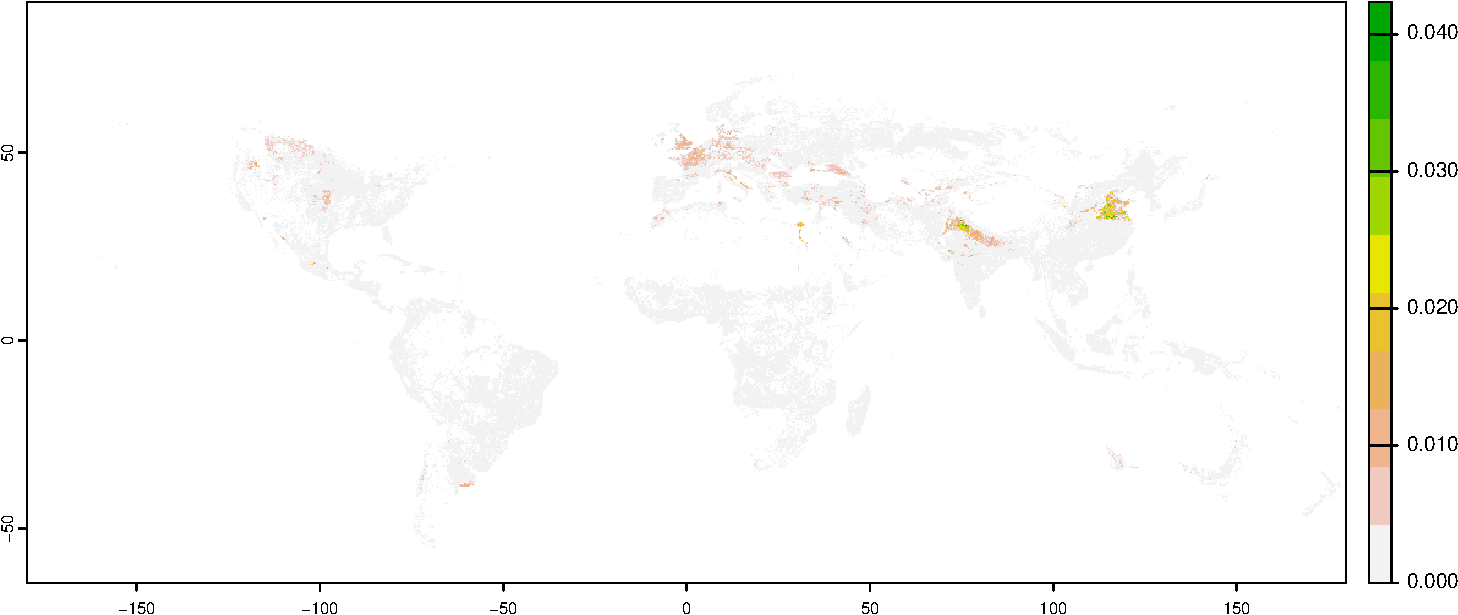
\includegraphics{global_n_files/figure-beamer/unnamed-chunk-6-1.pdf}

\linespread{2}

\linespread{0.5}

\begin{Shaded}
\begin{Highlighting}[]
\FunctionTok{writeRaster}\NormalTok{(wheat\_production\_Mt, }\AttributeTok{filename =} \StringTok{"./output/wheat\_production\_Mt.tif"}\NormalTok{, }
            \AttributeTok{overwrite=}\ConstantTok{TRUE}\NormalTok{, }\AttributeTok{gdal =} \FunctionTok{c}\NormalTok{(}\StringTok{"COMPRESS=DEFLATE"}\NormalTok{, }\StringTok{"TFW=YES"}\NormalTok{))}
\end{Highlighting}
\end{Shaded}

\linespread{2}
\end{column}
\end{columns}
\end{frame}

\begin{frame}{Task 2}
\protect\hypertarget{task-2}{}
\begin{itemize}[<+->]
\tightlist
\item
  Using the newly created raster and the GAUL shapefile of
  administrative borders, the production is aggregated to country level
  and exported to a csv file.
\end{itemize}
\end{frame}

\begin{frame}{Assumptions made}
\protect\hypertarget{assumptions-made}{}
\begin{itemize}[<+->]
\tightlist
\item
  The three input maps from the SPAM model for the year 2005 are global
  scale in raster format (5 arcminute spatial resolution):

  \begin{itemize}[<+->]
  \tightlist
  \item
    Estimates of yield (r\_y) in Kg/Ha,
  \item
    Physical area (r\_a) in Ha,
  \item
    Harvested area (r\_h) in Ha.
  \end{itemize}
\end{itemize}
\end{frame}

\begin{frame}{Issues}
\protect\hypertarget{issues}{}
\end{frame}

\begin{frame}{References}
\protect\hypertarget{references}{}
\renewcommand{\bibsection}{}
\bibliography{global_n.bib}

\linespread{0.5}

\linespread{2}
\end{frame}


\begin{frame}[allowframebreaks]{}
  \bibliographytrue
\end{frame}


\end{document}
